\documentclass[11pt,a4paper]{article}
\usepackage[utf8]{inputenc}
\usepackage[T1]{fontenc}
\usepackage[margin=2.3cm]{geometry}
\usepackage{amsmath,amssymb,bm}
\usepackage{booktabs}
\usepackage{graphicx}
\usepackage{float}
\usepackage{xcolor}
\usepackage{enumitem}
\usepackage{tcolorbox}
\usepackage{caption}
\captionsetup{font=small,labelfont=bf}
\graphicspath{{../../figures/models/md_unconditional/regimes/}}
\newtcolorbox{keybox}[1]{colback=blue!3,colframe=blue!45!black,title={#1},fonttitle=\bfseries,boxrule=0.6pt}
\newcommand{\E}{\mathbb{E}}

\title{\textbf{Speciation times, refined}\\[3pt]
\large Correlation-weighted theory, what ``under-confident'' means, and removing the classifier error}
\date{29 September 2026}

\begin{document}
\maketitle

\noindent This note follows \texttt{speciation\_explained.pdf}. It answers three questions:
\begin{enumerate}[nosep]
\item Can the profile theory be made more precise by weighting each revealed site's evidence with its correlations to
the other revealed sites, using the $n$-th root of $\prod(1-\rho)$ over its $n$ correlated partners? (\S1)
\item What exactly does ``the network is under-confident'' mean, and how large is the effect? (\S2)
\item Can we remove the error of the clade classifier, which is largest at the clade level? (\S3)
\end{enumerate}
Where things are:
\begin{itemize}[nosep]
\item code: \texttt{scripts/s14\_regimes\_refined.py} and new functions in \texttt{src/psg/regimes.py};
\item tests: \texttt{tests/test\_18\_regimes\_refined.py} (8 tests, all passing);
\item numbers: \texttt{evaluations/md\_unconditional/regimes\_refined*.json}.
\end{itemize}

\begin{keybox}{Summary}
\begin{itemize}[nosep,leftmargin=*]
\item \textbf{Classifier error was the main reason the clade speciation looked late.} Labelling clones with the exact
Bayes posterior of the true mixture moves the network's clade $k_S$ from 15.7 to \textbf{10.1} revealed sites. Family and
subfamily barely move.
\item \textbf{The network is under-confident, but only slightly.} Its class distribution behaves like the true one
shrunk towards uniform by a factor $\lambda\approx0.95$ at the clade level ($\approx0.98$ subfamily, $\approx1$
family). Correcting for this gives clade $k_S\approx$ \textbf{8.2}.
\item \textbf{Your correlation weighting improves the theory but cannot make it exact.} Within a class almost every pair
of sites is correlated, so the geometric mean acts as a roughly uniform discount ($w\approx0.71$--$0.77$). At clade
level it cuts the calibration error by a third and gives $k_S=9.7$, close to the network. No single-site weighting
calibrates the theory at every $k$.
\item Best estimates of the speciation points: family $\approx2$, subfamily $\approx5$, clade $\approx8$ revealed
sites, i.e.\ $t_S\approx0.97,\ 0.92,\ 0.86$.
\end{itemize}
\end{keybox}

%=====================================================================
\section{Weighting the log-sum by the correlations}
%=====================================================================
\subsection{The proposal}
The profile log-odds between classes $c$ and $c'$ is a sum of independent-looking terms:
\[
\Lambda=\sum_{i\in U}r_i(x^i),\qquad r_i(a)=\log\frac{f_{c,i}(a)}{f_{c',i}(a)} .
\]
If sites $i$ and $j$ are correlated within a class, the terms $r_i$ and $r_j$ partly repeat the same evidence, and the
sum counts it twice. The proposal is to multiply each term by a weight that shrinks when $i$ has correlated partners
among the \emph{revealed} sites:
\begin{equation}\label{eq:geo}
\Lambda_w=\sum_{i\in U}w_i\,r_i(x^i),\qquad
w_i=\Big[\prod_{j\in N_i(U)}(1-\rho_{ij})\Big]^{1/n_i},\qquad n_i=|N_i(U)| ,
\end{equation}
where $N_i(U)$ is the set of revealed sites $j\neq i$ that are correlated with $i$, and $w_i=1$ if there is none.
Equivalently, $w_i$ is the geometric mean of the $(1-\rho_{ij})$ over those partners. We apply the same weights to the
log-likelihood of every class, so the result is still a proper posterior:
$\log Q(c\mid x_U)=\log\pi_c+\sum_{i\in U}w_i\log f_{c,i}(x^i)-\text{normaliser}$.

\subsection{Which correlation $\rho_{ij}$?}
Residues are categorical, so we use the mutual information and turn it into a number between 0 and 1.
\begin{enumerate}[nosep]
\item \textbf{Within-class mutual information.} For each class $c$ at the level considered, with the pair frequencies
$f^c_{ij}(a,b)$ of its training sequences:
\[
\mathrm{MI}^c_{ij}=\sum_{a,b}f^c_{ij}(a,b)\log\frac{f^c_{ij}(a,b)}{f^c_i(a)\,f^c_j(b)} ,
\]
averaged over classes with weights equal to their sizes. \emph{Within} the class matters: the class label itself also
correlates sites, and that part is the signal we want, not redundancy.
\item \textbf{Bias correction.} With a finite sample, independent sites still show $\mathrm{MI}>0$ (about
$(q-1)^2/2N\approx0.02$ nats for $N=8000$ and $q=20$). We shuffle every column independently inside each class, which
destroys all correlations, recompute the MI, and subtract it. A second shuffle gives the noise level $\sigma$. A pair
counts as correlated (a ``partner'') if its corrected MI exceeds $5\sigma$.
\item \textbf{From MI to a correlation.} Linfoot's informational coefficient of correlation,
\[
\rho_{ij}=\sqrt{1-e^{-2\,\mathrm{MI}_{ij}}}\ \in[0,1) ,
\]
is exactly $|r|$ (the Pearson correlation) when the two variables are Gaussian. It is 0 for independent sites and tends
to 1 for copies.
\end{enumerate}
(Tested: a copied 4-state column gives $\mathrm{MI}=\log4$ and $\rho=\sqrt{1-1/16}$; an independent column gives
corrected $\mathrm{MI}\approx0$.)

\subsection{What the right weight would be}
To judge \eqref{eq:geo}, take the simplest case where the answer is known exactly. Suppose the evidence terms of the
revealed sites are jointly Gaussian with the same covariance in both classes, mean $\pm\bm m/2$ and correlation matrix
$R$ (unit variances for simplicity). The exact log-likelihood ratio of the vector $\bm e=(r_i)_{i\in U}$ is
\[
\Lambda_{\rm exact}=\bm m^\top R^{-1}\bm e .
\]
With independent sites, $R=I$ and every term gets weight 1. With correlations, the weights are the entries of
$R^{-1}\bm1$ (for equally informative sites).
\begin{itemize}[nosep]
\item \textbf{Two sites with correlation $r$:}
$R^{-1}\bm1=\frac{1}{1-r^2}\begin{pmatrix}1&-r\\-r&1\end{pmatrix}\begin{pmatrix}1\\1\end{pmatrix}=\frac1{1+r}\begin{pmatrix}1\\1\end{pmatrix}$,
so each weight is exactly $1/(1+r)$.
\item \textbf{$n+1$ sites, all correlated $r$ with each other:} each weight is $1/(1+nr)$.
\item \textbf{General small correlations:} $R^{-1}\approx I-(R-I)$, so $w_i\approx1-\sum_{j}r_{ij}$.
\end{itemize}
Compare the three simple formulas to first order in the correlations:
\begin{center}
\begin{tabular}{lll}
\toprule
weight & definition & first order\\
\midrule
geometric mean (your proposal) & $\big[\prod_{j}(1-\rho_{ij})\big]^{1/n_i}$ & $1-\frac1{n_i}\sum_j\rho_{ij}$ (the \emph{mean} $\rho$)\\
product & $\prod_{j}(1-\rho_{ij})$ & $1-\sum_j\rho_{ij}$\\
effective number & $1/\big(1+\sum_j\rho_{ij}\big)$ & $1-\sum_j\rho_{ij}$\\
exact (Gaussian) & $(R^{-1}\bm1)_i$ & $1-\sum_j\rho_{ij}$\\
\bottomrule
\end{tabular}
\end{center}
So for \emph{one} partner your formula is right to first order ($1-\rho\approx1/(1+\rho)$). With several partners, the
$n$-th root turns the sum into an average, and the discount no longer grows with the number of correlated partners. The
product and the effective number have the right first-order behaviour. One more property matters: for two perfect copies,
the product and the geometric mean both give weight $\approx0$ to \emph{both}, so the evidence disappears, whereas the
effective number gives $1/2$ each, which is right.

A caveat applies to all three: the correlation that matters is that of the evidence terms $r_i$, not of the residues.
$r_i$ is a function of $x^i$, so its correlation is at most the residue correlation, and usually smaller.

\subsection{Results}
Every variant is scored on 5000 held-out test sequences, for every $k$, with two criteria that need no theory:
\begin{itemize}[nosep]
\item \textbf{calibration gap} $\E\sum_cQ(c\mid x_U)^2-\E\,Q(\text{true }c\mid x_U)$. It is 0 for the true posterior
(proof in \S2.1), positive if $Q$ is over-confident, negative if under-confident;
\item \textbf{log-loss} $\E[-\log Q(\text{true }c\mid x_U)]$: lower is better.
\end{itemize}
\begin{center}\small
\begin{tabular}{llccc}
\toprule
level & weighting & log-loss & mean $|$gap$|$ & $k_S$\\
\midrule
family & none (independent sites) & \textbf{0.071} & \textbf{0.001} & 2.1\\
 & geometric mean of $(1-\rho)$ & 0.073 & 0.004 & 3.0\\
 & effective number, $\rho^2$ & 0.076 & 0.007 & 2.3\\
 & best uniform weight ($w=0.95$) & \textbf{0.071} & \textbf{0.001} & 2.2\\
\midrule
subfamily & none & 0.360 & 0.019 & 4.9\\
 & geometric mean of $(1-\rho)$ & \textbf{0.340} & \textbf{0.012} & 6.5\\
 & effective number, $\rho^2$ & 0.367 & 0.041 & 6.9\\
 & best uniform weight ($w=0.70$) & 0.343 & 0.013 & 6.9\\
\midrule
clade & none & 0.809 & 0.065 & 7.4\\
 & geometric mean of $(1-\rho)$ & 0.733 & 0.043 & 9.7\\
 & effective number, $\rho^2$ & \textbf{0.708} & 0.044 & 13.3\\
 & best uniform weight ($w=0.55$) & 0.716 & \textbf{0.032} & 13.4\\
\bottomrule
\end{tabular}
\end{center}
The product and the effective number with $\rho$ itself fail at every level. For clades, their log-loss is 2.6 and 1.0
and their commitment never reaches $1/2$. With $\rho^2$ the product also fails (clade log-loss 1.28).

\begin{figure}[H]
\centering
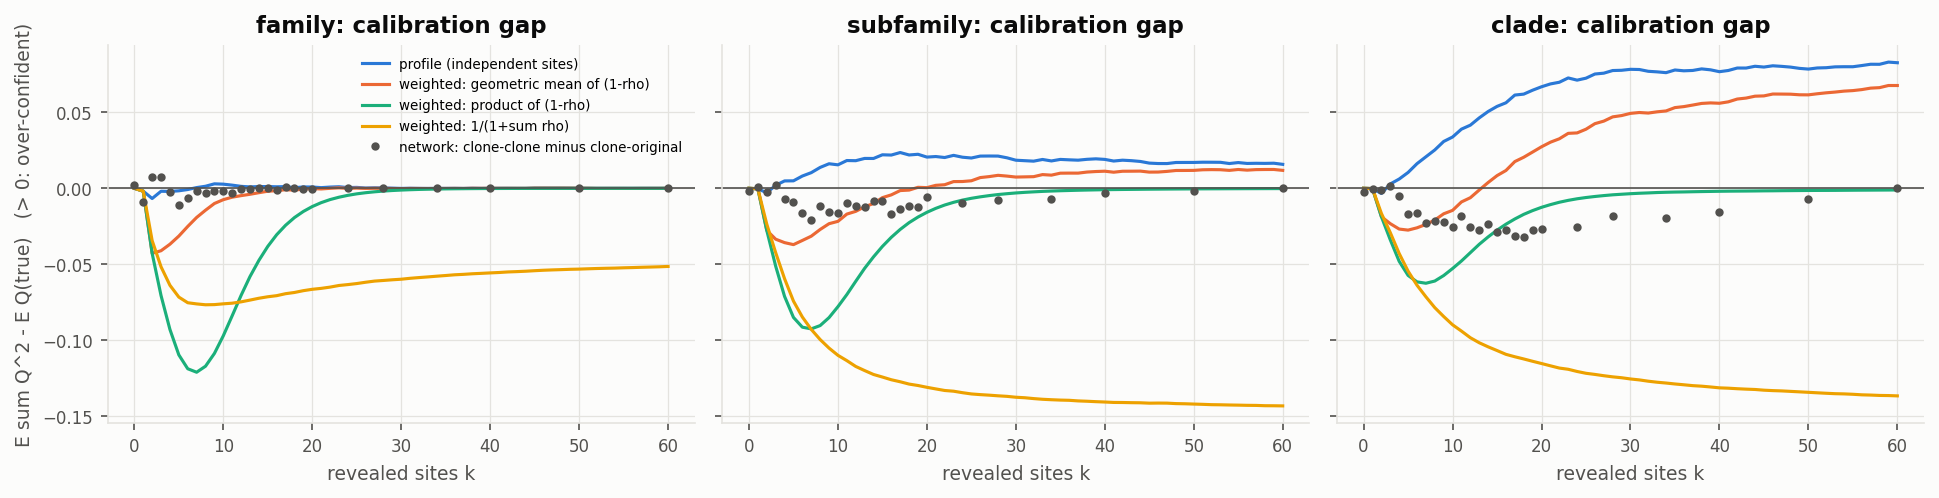
\includegraphics[width=\textwidth]{refined_calibration.png}
\caption{Calibration gap against the number of revealed sites (positive: over-confident). Blue: independent-site
profile. Red: your geometric-mean weighting. Green and yellow: product and effective number with $\rho$. Dots: the
network (\S2).}
\label{fig:cal}
\end{figure}

\paragraph{What we learn.}
\begin{enumerate}[nosep]
\item \textbf{Within a class, almost every pair of sites is correlated}: 1730--1770 of the 1770 pairs pass the $5\sigma$
threshold, with mean $\rho\approx0.23$--$0.28$. The couplings live on only 179 contacts, but they propagate: $i$--$j$ and
$j$--$k$ in contact make $i$ and $k$ correlated. At the family and subfamily levels the class is also a mixture of
sub-classes, which correlates everything. So every site has almost every other revealed site as a partner.
\item \textbf{Your weighting therefore acts as a nearly uniform discount}: the average weight is 0.71 (family), 0.75
(subfamily) and 0.77 (clade), almost independent of $k$. That is too strong when few sites are revealed, since one
partner already costs 25\%, and too weak when many are, since the discount does not grow. Fig.~\ref{fig:cal} (red) shows
exactly this: under-confident for $k\lesssim10$, over-confident beyond.
\item \textbf{The formulas whose discount grows with the number of partners over-correct}, because $\sum_j\rho_{ij}$ over
$\sim k$ partners of $\rho\approx0.25$ quickly exceeds 1. The residue correlation over-states the evidence
correlation (the caveat of \S1.3). Using $\rho^2$ helps the effective number at the clade level but hurts it at the
subfamily level.
\item \textbf{No single-site weighting is calibrated everywhere.} The best constant weight leaves a clade gap of 0.03.
The rest of the error is not double counting: the profile also ignores the \emph{differences in couplings} between
clades, which carry class information that no re-weighting of site terms can recover.
\item \textbf{Overall, your geometric mean is the best simple variant.} It is best at the subfamily level and much
better than no weighting at the clade level (gap $-34\%$, log-loss $-9\%$). It is slightly worse only at the family level,
where the profile was already calibrated.
\end{enumerate}

%=====================================================================
\section{What ``under-confident'' means}
%=====================================================================
\subsection{Definitions and the test}
Fix a partial sequence $x_U$. Two distributions over the class $y$ of its completion matter:
\begin{itemize}[nosep]
\item $P(y\mid x_U)$, the \textbf{truth}: the class distribution of true sequences that agree with $x_U$;
\item $Q(y\mid x_U)$, the \textbf{network's}: the class distribution of the network's completions of $x_U$.
\end{itemize}
We measure two agreements, starting from masked \emph{true} sequences $x_0$:
\begin{align*}
\text{clone--clone:}\quad&\Pr[\text{two clones share the class}]=\E_{x_U}\sum_yQ(y\mid x_U)^2 ,\\
\text{clone--original:}\quad&\Pr[\text{a clone shares the class of }x_0]=\E_{x_U}\sum_yQ(y\mid x_U)\,P(y\mid x_U) .
\end{align*}
The second line holds because, given $x_U$, the original $x_0$ is itself a draw from the truth, independent of the
clones. If $Q=P$ the two lines are equal. Their difference is
\[
\text{clone--original}-\text{clone--clone}=\E\sum_yQ(y)\big[P(y)-Q(y)\big].
\]

\subsection{A one-parameter model: shrinkage towards uniform}
Suppose the network's distribution is the truth pulled towards the uniform distribution $u(y)=1/K$:
\[
Q=\lambda P+(1-\lambda)u .
\]
Then $P-Q=(1-\lambda)(P-u)$. Using $\sum_yu(y)(P(y)-u(y))=0$:
\[
\sum_yQ(P-Q)=(1-\lambda)\Big[\lambda\sum_yP(P-u)+(1-\lambda)\sum_yu(P-u)\Big]=\lambda(1-\lambda)\Big(\sum_yP^2-\tfrac1K\Big).
\]
Since $\sum_yP^2\ge1/K$, this is \textbf{positive for $0<\lambda<1$}. That is \textbf{under-confidence}: $Q$ is flatter
than $P$, and a clone agrees with the original more often than with another clone. It is \textbf{negative for
$\lambda>1$}: over-confidence, $Q$ sharper than $P$.

\emph{Example.} $P=(0.8,\,0.2)$ and $\lambda=0.5$ give $Q=(0.65,\,0.35)$. Clone--clone is $0.65^2+0.35^2=0.545$ and
clone--original is $0.8\times0.65+0.2\times0.35=0.590$. The difference $0.045$ equals $0.5\times0.5\times(0.68-0.5)$.

\paragraph{Estimating $\lambda$ and the true commitment.} The model also gives
$\sum Q^2-\frac1K=\lambda^2\big(\sum P^2-\frac1K\big)$ and $\sum PQ-\frac1K=\lambda\big(\sum P^2-\frac1K\big)$. Dividing
and squaring:
\[
\lambda=\frac{\text{cc}-1/K}{\text{co}-1/K},\qquad
\sum_yP^2=\frac1K+\frac{(\text{co}-1/K)^2}{\text{cc}-1/K},
\]
where cc and co are the measured clone--clone and clone--original agreements. This gives an estimate of the \emph{true}
commitment curve from the network's clones, corrected for its under-confidence. (It treats $\lambda$ as the same for
all $x_U$, so it is an approximation.)

\subsection{Measured (exact soft labels, \S3)}
\begin{center}\small
\begin{tabular}{lcccc}
\toprule
$\lambda$ at $k=$ & 2 & 5 & 10 & 20\\
\midrule
family & 1.02 & 0.98 & 1.00 & 1.00\\
subfamily & 0.99 & 0.98 & 0.97 & 0.99\\
clade & 0.99 & 0.94 & 0.95 & 0.96\\
\bottomrule
\end{tabular}
\qquad
\begin{tabular}{lccc}
\toprule
clade, $k=$ & 5 & 10 & 20\\
\midrule
clone--clone & 0.330 & 0.501 & 0.695\\
clone--original & 0.347 & 0.527 & 0.722\\
\bottomrule
\end{tabular}
\end{center}
\paragraph{What it means.} From a partial sequence, the network's completions land in the \emph{sibling} clade (or
subfamily) a little more often than true sequences with the same revealed residues do. It has not extracted all of the
clade-specific evidence the revealed residues contain. At the clade level it keeps about 95\% of the true confidence.
The effect is the same as in Part~III (within-family correlations about 10\% too weak, per-clade $r_C$ 0.764 against
0.828): the fine, clade-specific signal ($\sigma_h=0.3$, $\sigma_J=0.15$ in the tree) is learned only partly.

\paragraph{Two further pieces of evidence.}
\begin{itemize}[nosep]
\item \textbf{The network's own samples are more ambiguous.} The exact posterior of a complete sequence gives
$\E\sum_cP(c\mid x)^2=0.954$ for true sequences but only 0.868 for network samples (clade level; 0.999 vs 0.982 for
subfamilies). Network samples sit more often \emph{between} two sibling clades.
\item \textbf{The network is self-consistent.} Starting from masked \emph{network samples}, clone--clone and
clone--original agree within 0.01 at every level and $k$. This is expected if the network's conditionals come from a
single joint distribution, which a masked-diffusion network does not guarantee. So the gap measured on true sequences is
a gap between the network and the truth, not internal inconsistency.
\end{itemize}

%=====================================================================
\section{Removing the classifier error}
%=====================================================================
\subsection{Why the classifier biases the clade level most}
Until now every clone was labelled by the clade with the highest pseudo-likelihood. On labelled test sequences this is
right for 100\% of families, 99.4\% of subfamilies but only 91.5\% of clades. Near the boundary between two sibling clades,
a completion that differs in a few residues can flip the label. That adds noise to clone agreement, lowers the curve,
and delays the $1/2$-crossing. Sibling clades differ least, so the effect is largest there.

The right label is the \textbf{latent} class, the model the sequence was drawn from. For a complete sequence $x$ it is
known only in probability:
\[
P(c\mid x)=\frac{e^{-E_c(x)}/Z_c}{\sum_{c'}e^{-E_{c'}(x)}/Z_{c'}}\qquad(\text{equal priors}).
\]
This needs the partition functions $Z_c$, which the pseudo-likelihood avoided.

\subsection{Partition functions by thermodynamic integration}
Introduce a coupling strength $\lambda\in[0,1]$ in each clade model:
\[
E_\lambda(x)=-\sum_ih_i(x^i)-\lambda\sum_{i<j}J_{ij}(x^i,x^j).
\]
(This $\lambda$ is unrelated to the shrinkage factor of \S2.)
\begin{enumerate}[nosep]
\item At $\lambda=0$ the sites are independent, so $\log Z_0=\sum_i\log\sum_ae^{h_i(a)}$ exactly.
\item Differentiating $\log Z_\lambda=\log\sum_xe^{-E_\lambda(x)}$:
\[
\frac{d\log Z_\lambda}{d\lambda}=\frac{\sum_x\big(\sum_{i<j}J_{ij}\big)e^{-E_\lambda(x)}}{Z_\lambda}
=\Big\langle\sum_{i<j}J_{ij}(x^i,x^j)\Big\rangle_\lambda ,
\]
an average that Gibbs sampling at strength $\lambda$ estimates.
\item Integrating: $\log Z_1=\log Z_0+\int_0^1\big\langle\sum_{i<j}J_{ij}\big\rangle_\lambda\,d\lambda$, with Simpson's rule on
21 values of $\lambda$ and 1000 GPU chains warm-started from one $\lambda$ to the next.
\item The integral is computed going up and going down in $\lambda$. Half their difference estimates the error: at most
0.095 nats over the 18 clades. A 5$\times$ longer run on clade 0 gives $\log Z=340.07$ against 340.10.
\end{enumerate}
\texttt{test\_18} checks this against exact enumeration on small models (error $<0.02$).

\paragraph{Validation on the labelled test set.} If the $Z_c$ are right, the posterior is calibrated:
$\E\sum_cP^2=\E P(\text{true }c)$, because the true labels are draws from it.
\begin{center}\small
\begin{tabular}{lccc}
\toprule
 & family & subfamily & clade\\
\midrule
accuracy, exact posterior (Bayes-optimal) & 1.000 & 1.000 & \textbf{0.969}\\
accuracy, pseudo-likelihood classifier & 1.000 & 0.994 & 0.915\\
$\E\sum_cP(c\mid x)^2$ & 1.000 & 0.999 & 0.954\\
$\E\,P(\text{true }c\mid x)$ & 1.000 & 0.999 & 0.954\\
\bottomrule
\end{tabular}
\end{center}
The last two rows agree to 3 decimals, so the $Z_c$ are right. Even the best possible classifier is wrong on 3.1\% of
clades: sibling clades genuinely overlap, and a complete sequence leaves clade commitment 0.954, not 1.

\subsection{Soft-label cloning}
Label each clone $a$ by its whole posterior vector $R_a(y)=P(y\mid\text{clone }a)$ instead of a hard label, and measure,
for $C$ clones of the same $x_U$,
\[
\widehat\phi=\frac1{C(C-1)}\sum_{a\neq b}\ \sum_yR_a(y)R_b(y).
\]
\emph{Why this is exact.} With the exact denoiser, a clone is a draw from $P(x_0\mid x_U)$, so
$\E[R_a(y)\mid x_U]=\sum_{x_0}P(x_0\mid x_U)P(y\mid x_0)=P(y\mid x_U)$, the latent-class posterior. Two clones are
independent given $x_U$, so $\E[\sum_yR_aR_b\mid x_U]=\sum_yP(y\mid x_U)^2$. No classifier is involved.

At $k=L$ the curve ends at the ceiling $\E\sum_yP(y\mid x)^2$ (0.954 for clades), not at 1. The normalised commitment is
therefore $\psi=(\phi-\phi_0)/(\phi_{\rm ceiling}-\phi_0)$, and $k_S$ is where it crosses $1/2$.

\subsection{Results}
\begin{center}\small
\begin{tabular}{lcccc}
\toprule
 & \multicolumn{2}{c}{from held-out true $x_t$} & \multicolumn{2}{c}{from the network's own paths}\\
$k_S$ & classifier labels & exact soft labels & classifier labels & exact soft labels\\
\midrule
family & 1.93 & 1.93 & 1.95 & 1.94\\
subfamily & 5.83 & 5.36 & 5.50 & 4.91\\
clade & 15.7 & \textbf{10.1} & 17.7 & \textbf{8.7}\\
\bottomrule
\end{tabular}
\end{center}
\begin{figure}[H]
\centering
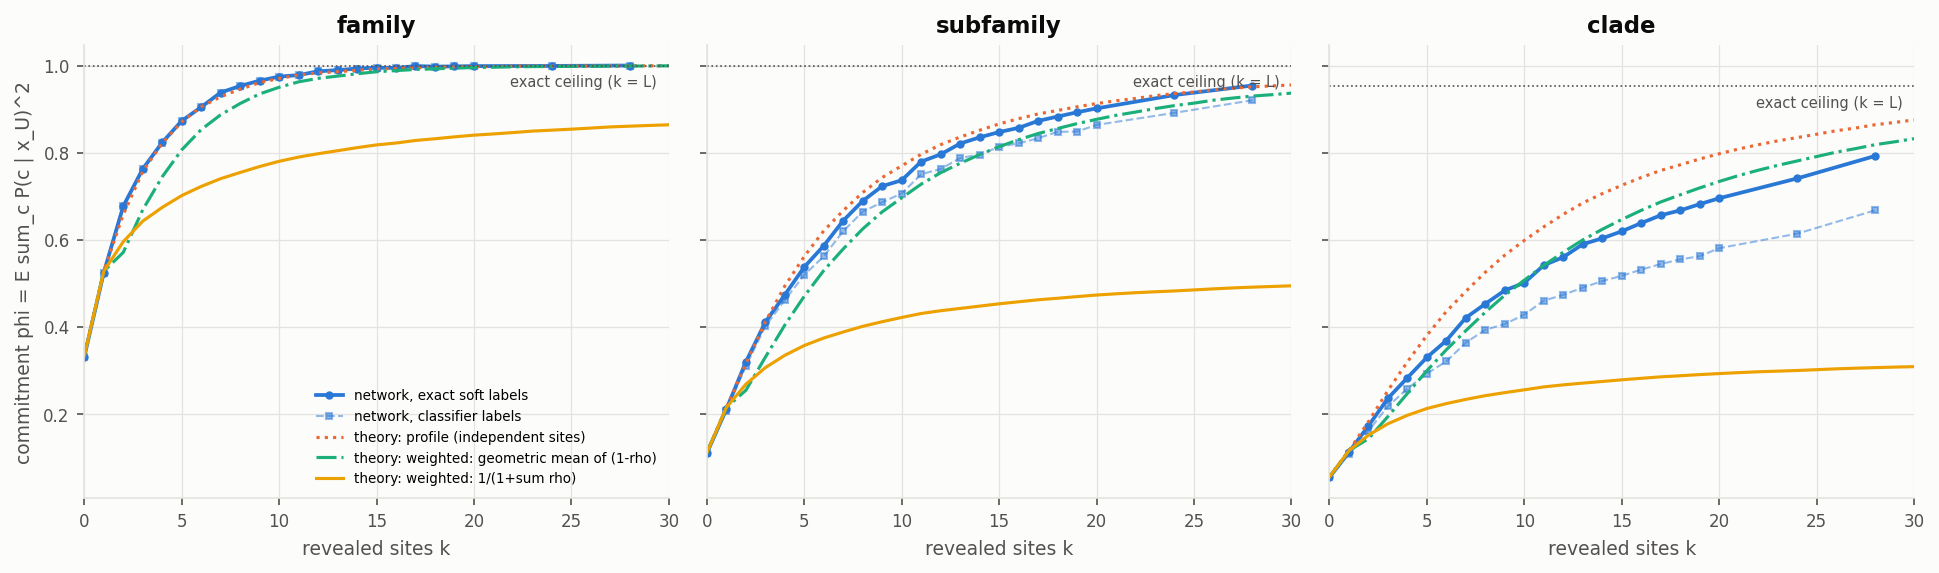
\includegraphics[width=\textwidth]{refined_speciation.png}
\caption{Commitment $\phi=\E\sum_cP(c\mid x_U)^2$ (not normalised). Dark blue: the network with exact soft labels.
Light blue: the same clones with classifier labels. Dotted, dash-dotted, solid: profile theory without weighting, with your
geometric-mean weighting, and with the effective number. Grey: the exact ceiling at $k=L$.}
\label{fig:spec}
\end{figure}
Classifier noise was responsible for most of the apparent clade delay. With soft labels, the network's clade curve lies
between the unweighted profile theory (over-confident) and your weighted one, and it follows the weighted theory closely
up to $k\approx12$ (Fig.~\ref{fig:spec}).

%=====================================================================
\section{Updated speciation points}
%=====================================================================
\begin{center}\small
\begin{tabular}{lccc}
\toprule
$k_S$ (revealed sites) & family & subfamily & clade\\
\midrule
profile theory, independent sites (over-confident) & 2.1 & 4.9 & 7.4\\
profile theory, your geometric-mean weighting & 3.0 & 6.5 & 9.7\\
profile theory, best uniform weight (calibrated on average) & 2.2 & 6.9 & 13.4\\
network, classifier labels (previous result) & 1.9 & 5.8 & 15.7\\
network, exact soft labels & 1.9 & 5.4 & 10.1\\
network, soft labels, corrected for under-confidence (\S2.2) & \textbf{2.0} & \textbf{5.0} & \textbf{8.2}\\
\bottomrule
\end{tabular}
\end{center}
How to read the range:
\begin{itemize}[nosep]
\item A theory that is calibrated but uses \emph{less} information than the truth commits \emph{more slowly}. If
$Q=\E[P\mid\text{less information}]$, Jensen's inequality gives $\E\sum Q^2\le\E\sum P^2$. The calibrated profile
(13.4 for clades) ignores the coupling differences between clades, so it is an \emph{upper} bound on the true $k_S$.
\item The network with soft labels is slightly under-confident, so its 10.1 is also an upper bound. Correcting for the
shrinkage gives 8.2.
\item The independent-site profile is over-confident, so its 7.4 is too early.
\end{itemize}
Our best estimates are therefore family $\approx2$, subfamily $\approx5$ and clade $\approx8$ revealed sites, i.e.\
$t_S\approx0.97,\ 0.92,\ 0.86$. The cascade stands. With these values, the collapse of the empirical denoiser
($k_C=6.2$, unchanged) still falls between subfamily and clade speciation.

\end{document}
